\chapter{La Composition des services web}
%% TODO Introduire la notion de la composition et le plan du chapitre

% Dans le chapitres précédent, nous avons étudiés la description, la
% publication,  la découverte et la sélection de services Web
% élémentaire. L'autre concept fondamentale % est la composition des
% services web.


  
%   % The other fundamental concept is web service composition which
% sometimes overlaps or will merge with the process of WS
% discovery. WS composition is a mechanism of combining two or more
% basic services into a possibly complex service. It is used to solve
% complex problems by combining available basic services. It helps to
% accelerate rapid application development and facilitate service
% reuse from developer perspective % and from user perspective it
% increases complex service consumption. As mentioned earlier a
% composite service can be regarded as a combination of services invoked
% in % a predefined order and executed as a whole and that has more
% functionality than its components. WS composition is needed because
% finding a right service provider for the request is not an easy task
% on fast growing WWW sometimes it is even % impossible. Thus WS
% composition becomes necessary and inevitable. Composing WS from
% existing ones is an effective method to fill this gap.\cite{Omer2011}

%   Dans ce chapitre, nous présentons dans un premier temps les
% définitions et les types de composition de services Web présents dans
% la littérature. Ensuite, nous étudions .....
%   Enfin, un ensemble de travaux proposent des approches de la
% composition dynamiques des services web sémantiques.

\newpage

  \section{Définition et stratégies de composition}
  \label{sec:defin-et-caract}

  Cette section a pour but d'exposer, d'une part, quelques définitions
  et objectifs de la composition des services Web proposées par la
  communauté, et d'autre part, les différents types et mécanismes de
  composition selon différents points de vue rencontrés dans la
  littérature.
  
    \subsection{Définitions}
    \label{sec:definitions}

    Martin \emph{et al.} \cite{martin2004owl} définissent
    la composition comme étant \emph{``le processus de sélection, de
      combinaison et d'exécution de services en vue
      d'accomplir un objectif donné''}.
    % TODO discussion de la définition.

    Selon S. Dustdar et W. Schreiner \cite{dustdar2005survey} :
    \emph{`` L'infrastructure de base des services Web suffit pour la
      mise en œuvre d'interactions simples entre un client et un
      service Web. Si la mise en œuvre d'une application métier
      implique l'invocation d'autres services web, il est nécessaire
      donc de combiner les fonctionnalités de plusieurs services
      web. Dans ce cas, nous parlons d'une composition de services
      Web''}.

    % TODO discussion.
    En d'autre terme, La composition de services Web désigne une
    opération qui consiste à construire de nouvelles applications ou
    services appelés \textbf{services composites} ou agrégats par
    l'assemblage ou l'agrégation de services existants nommés
    \textbf{services atomiques} ou élémentaires.

    Medjahed \cite{medjahed2004thesis}de ça part a défini un service
    Web composite commme un \emph{``conglomérat de sous-traitance
      services Web (services appelés participants) travaillant en
      tandem pour offrir un service à valeur ajoutée.''}\\

    La composition de services Web vise essentiellement quatre
    objectifs \cite{driss2011approche}:
    \begin{enumerate}
      \item Créer de nouvelles fonctionnalités en combinant des services
        déjà existants.
      \item Résoudre des problèmes complexes auxquels aucune solution\\
        n'a été trouvée.
      \item collaborer plusieurs entreprises ensemble.
      \item Optimiser et améliorer une fonctionnalité existante.
    \end{enumerate}

    % le processus générale de composition
    \subsection{Cycle de vie d'une composition }
    \label{sec:cycle-de-vie+exigences}
    % TODO: introduce
    % Dans cette sous-section, nous discutons du cycle de vie de la
    % composition de services Web, qui est divisé en quatre phases. Pour
    % chaque phase, un ensemble d'exigences est identifié.

    % Compte tenu de la nature très dynamique et distribué des
    % environnements de services Web, certaines exigences doivent être
    % respectées afin de parvenir à la composition de services Web
    % avec succès. Dans cette sous-section, nous identifions plusieurs
    % exigences pour chaque phase du cycle de vie d'un composition des
    % services Web.

    Comme l'illustre la figure, le cycle de vie de la composition de
    services Web comprend quatre phases \cite{sheng2014web}: la phase
    de \textit{définition}, La phase de \textit{sélection}, la phase
    de \textit{déploiement} et la phase d'\textit{exécution}:.

    \begin{figure}[h]
    \centering
    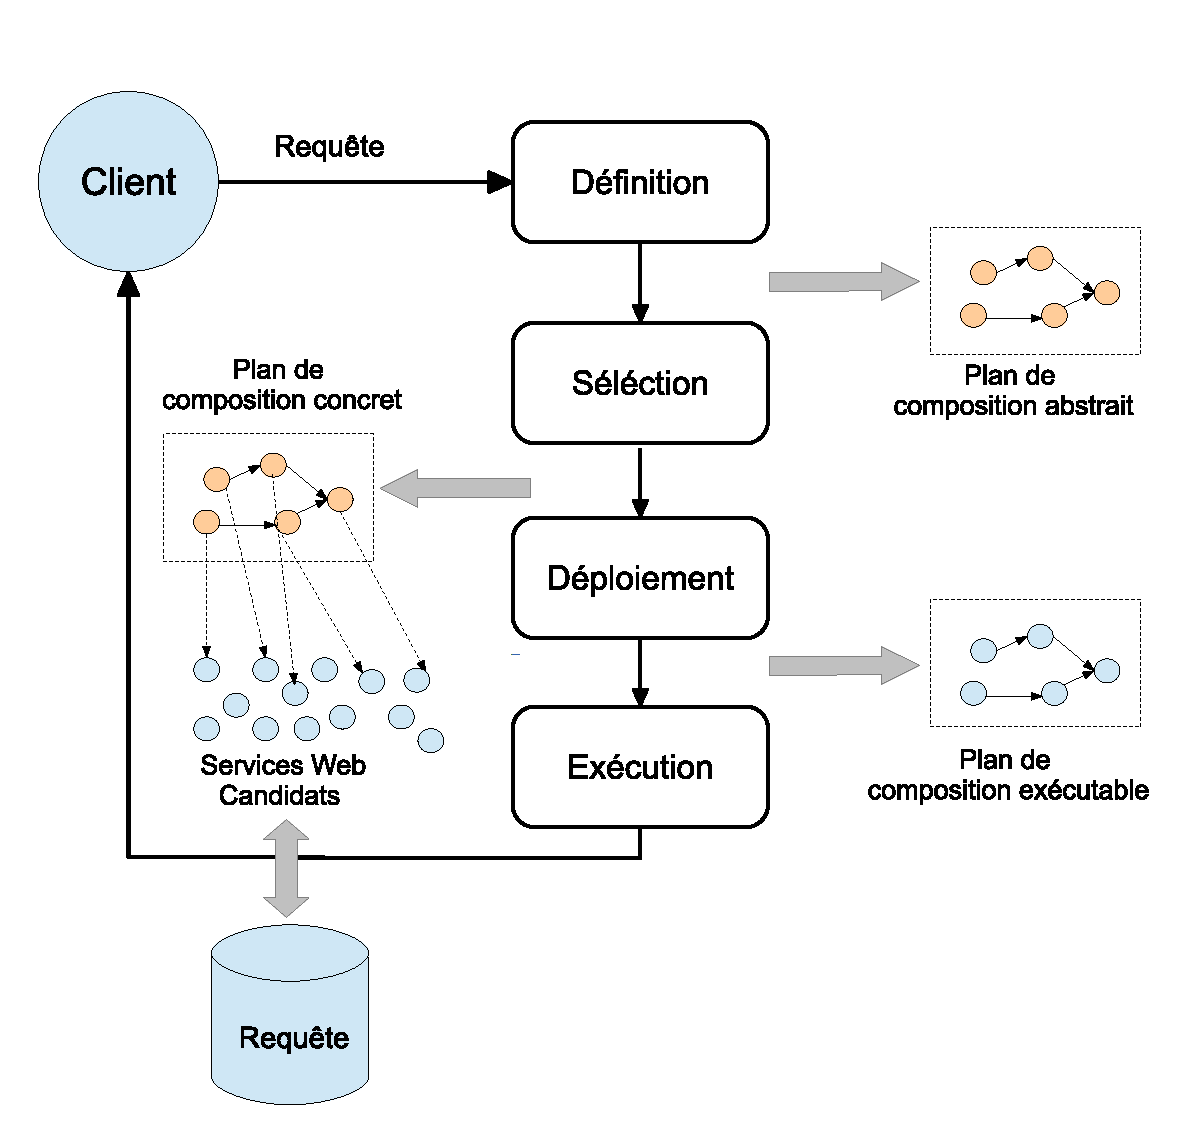
\includegraphics[width=0.9\textwidth]{figs/composition-life-cycle.eps}
    % TODO translate the figure
    % TODO reference the fig
    \caption{Cycle de vie d'une composition des services
      \cite{sheng2014web}.}
    \label{fig:composition-life-cycle.eps}
\end{figure}

%%% Local Variables:
%%% mode: latex
%%% TeX-master: "../main"
%%% End:

    % \newpage
    \SpecialItem
    \begin{description}
    \item[La phase de définition] Pendant cette phase, le client de
      service spécifie les exigence de composition des services en
      termes des besoins et des préférences pour le service
      composite. l'exigence est ensuite \textit{décomposé}, soit
      semi-automatique ou automatique, dans un modèle de
      \textbf{processus abstrait}(ce est à dire, le service composite
      abstraite), qui spécifie un ensemble d'activités, le contrôle et
      le flux de données entre eux, la qualité de service
      \acrshort{qos} et la gestion des exceptions.

      %% TODO: REWRITE
    \item[La phase de séléction.] Dans cette phase, pour chaque
      activité dans le service composite, les services Web appropriés
      qui répondent aux exigences de l'activité sont situés en
      cherchant sur le registre de service, sur la base des
      informations contenues dans les documents de description de
      service publiées. Il est probable que plus d'un service de
      candidat de répondre aux exigences. Par conséquent, le meilleur
      le service identifié doit être sélectionné. Après tous les
      services Web requis sont identifiés et liés aux activités
      correspondantes, le service composite construit est produite.

    \item[La phase de déploiement.]Dans cette phase, le service
      composite construit est déployé pour permettre son
      instanciation et l'invocation par les utilisateurs finaux. Le
      résultat de cette phase est le service composite exécutable.

    \item[La phase d'exécution.] Dans cette phase, l'instance de
      service composite est créé et exécuté par le moteur
      d'exécution, qui est aussi responsable de l'invocation des
      composants de service atomiques. Pendant l'exécution de
      l'instance de service composite, les tâches de surveillance, y
      compris le suivi d'exécution, mesure de la performance et la
      gestion des exceptions, doivent être effectuées.
    \end{description}
    \newpage
    \subsection{Procédés de coordination}
    \label{sec:proc-de-coord}
    % It should be noted that these models are not used exclusively:
    % one approach can implement more than one models at the same
    % time.\cite{baryannis2010} %% TODO: translate
    Nous distinguons deux méthodes utilisés pour décrire la
    composition de services dans un flot de processus métier:
    l'\emph{orchestration} de services et la \emph{chorégraphie} des
    services. Ces deux procédés de coordination décrivent deux aspects
    de création des processus métiers à partir des services Web
    composites \cite{peltz2003web}.
    %% Introduire la notion d'un procédé de coordination
    \textbf{Un procédé} est représenté par un graphe orienté
    d'activités ou un flot de contrôle qui donne l'ordre d'exécution
    des activités et la logique de coordination des services. Chaque
    activité représente une fonctionnalité réalisée concrètement par
    un service \cite{chollet2009orchestration}.

    La figure \ref{fig:orchestration-vs-choregraphie} illustre ces
    deux approches en conjonction.
    % orchestration vs chorégraphie
    \begin{figure}[h]
    \centering
    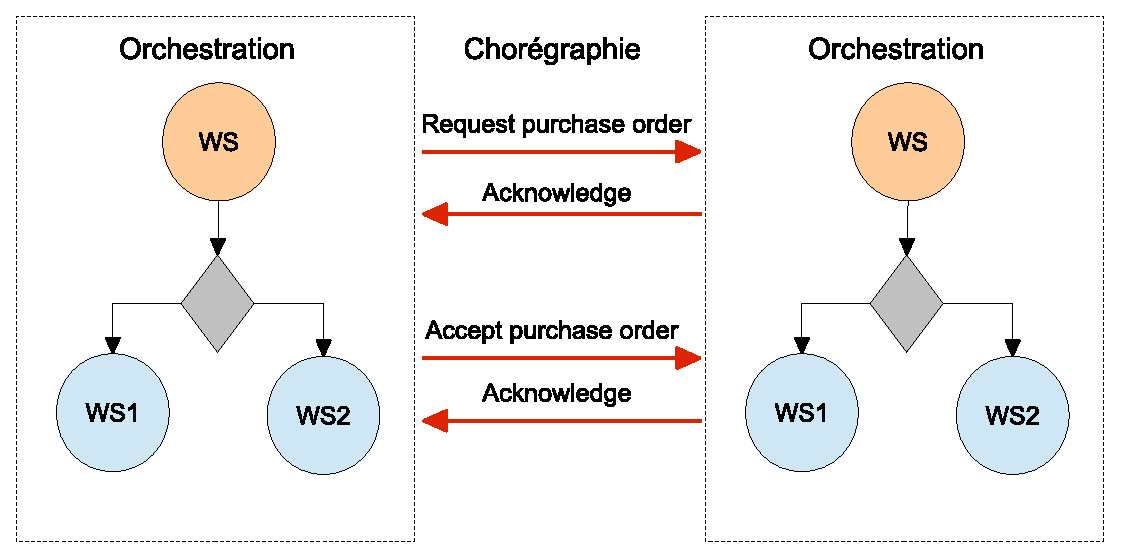
\includegraphics[width=1\textwidth]{figs/orchestration-vs-choregraphie.eps}
    \caption{Orchestration vs Chorégraphie selon Peltz
      \cite{peltz2003web}.}
    \label{fig:orchestration-vs-choregraphie}
\end{figure}       

      \subsubsection{Orchestration}
      \label{sec:orchestration-sec}
      Selon Sonia \emph{et al.} \cite{jamal2005environnement}:
      \emph{``L'orchestration des services Web permet de définir
        l'arranegement et l'enchaînement de ces services selon un
        canevas bien défini. Elle décrit la manière par laquelle les
        services peuvent interagir ensemble tout en incluant l'ordre
        d'exécution des différentes interactions''}.

      Barros \emph{et al.} \cite{barros2006standards} définissent
      l'orchestration comme un ensemble de processus exécutés dans un
      ordre prédéfini afin de répondre à un but
      \cite{lopez2008selection}. Ce type de composition se base sur un
      procédé métier exécutable permettant de décrire d'enchaînement
      et les interactions des différents services basiques collaborant
      dans une composition.
      
      L'orchestration offre \textbf{une vision centralisée} de
      contrôle, le procédé est toujours contrôlé par l'un des
      partenaires métiers. Ce dernier joue le rôle d'un chef
      d'orchestre qui se charge d'appeler les services de la
      composition suivant l'ordre d'exécution déjà défini par le
      processus métier. Le principe de l'orchestration est illustré
      par La figure \ref{fig:orchestration}.
      %TODO: citer qulques languages d'orchestration
      %TODO: les avantages et les inconvénients

      \subsubsection{Chorégraphie}
      \label{sec:choregraphie-sec}
      Selon Sonia \emph{et al.} \cite{jamal2005environnement} :
      \emph{`` La chorégraphie permet de tracer la séquence de
        messages échangés dans un contexte de composition de services
        Web. Elle est typiquement liée à la description de
        conversations existantes entre les services tout en impliquant
        plusieurs parties, incluant les clients, les fournisseurs et
        les partenaires''}.

      D'après Barros \emph{et al.} \cite{barros2006standards}, la
      chorégraphie permet de décrire la composition comme un moyen
      d'atteindre un but commun en utilisant un ensemble de services
      Web. La collaboration entre chaque service Web de la collection
      (faisant partie de la composition) est décrite par des flots de
      contrôle \cite{lopez2008selection}.

      La chorégraphie offre \textbf{une vision décentralisée} et
      \textbf{globale} du système et exprime une vue d'ensemble des
      services interagissant dans le cadre d'une composition de
      services. Selon Peltz \cite{peltz2003web}, la chorégraphie
      illustre les différants échanges de messages entre les
      participants. Le principe de la chorégraphie est illustré par la
      figure \ref{fig:choregraphie}.
      %TODO: citer qulques languages de chorégraphie.
      %TODO: les avantages et les inconvénients.

    \subsection{Stratégies de composition}
    \label{sec:types-de-composition}
    %TODO: re-write
    Un modèle de composition de service peut être relativement
    complexe. Il requiert la description et l'organisation de
    l'interaction entre les services et nécessite la gestion de
    plusieurs aspects comme les échanges de données entre les
    services, les pannes ou erreurs éventuelles, le contexte
    d'interaction, le degré d'automatisation des tâches, etc\dots
    
    Il existent une variété de spécifications, de langages et
    d'approches formelles développées par la littérature concernant la
    composition. Ces techniques sont également classés en fonction de
    différents dimensions, et selon les travaux effectués dans le
    champ des services web, les définitions des types de composition
    diffèrent d'une communauté de l'autre.
 
    Barros \emph{et al.} \cite{barros2006standards} classent la
    composition des services Web en trois catégories : la composition
    comportementale, l'orchestration et la chorégraphie, à l'instar de
    Barros \emph{et al.}, Peltz \cite{peltz2003web} considère que les
    deux dernières \textit{(orchestration, chorégraphie)}.

    \begin{figure}[h]
    \centering
    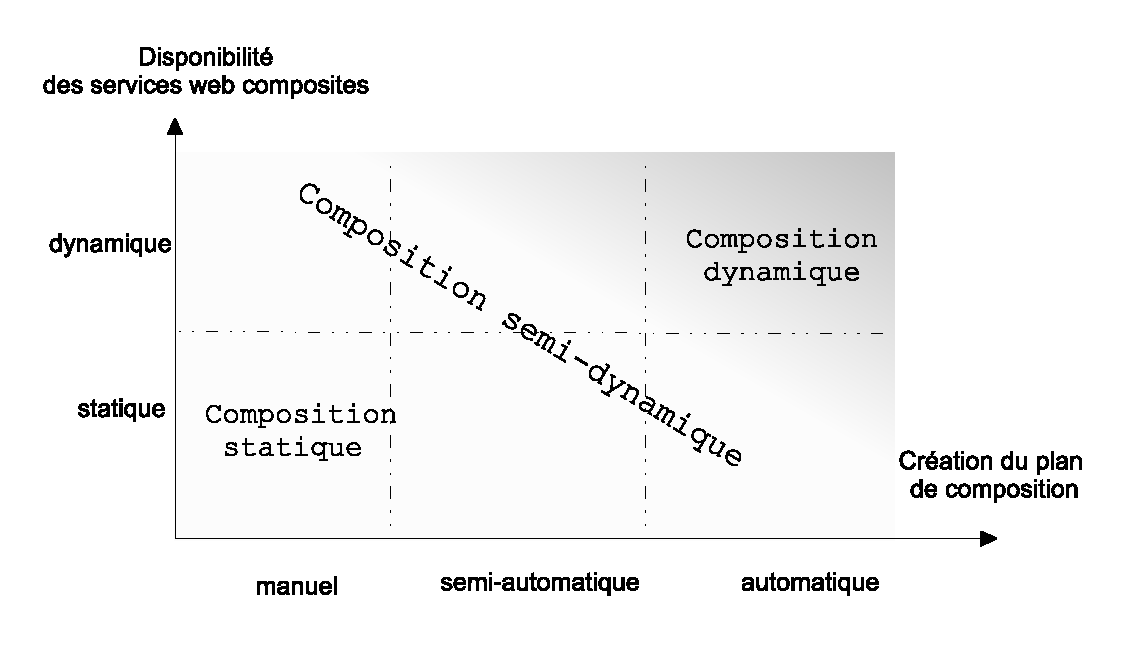
\includegraphics[width=1.1\textwidth]{figs/static-vs-dynamic-composition.eps}
    \caption{Classification des stratégies de composition
      \cite{fluegge2006challenges}.}
    \label{fig:static-vs-dynamic-composition}
\end{figure}
%%% Local Variables: 
%%% mode: latex
%%% TeX-master: "../main"
%%% End: 


    D'une autre façon, Fluegge \emph{et
      al.}\cite{fluegge2006challenges} dans une analyse de l'état de
    l'art considèrent l'orchestration et la chorégraphie comme des
    modèles d'exécution appliqués dans le contexte d'une
    composition. Il distingue trois stratégies de composition selon la
    disponibilité des services Web composites lors de composition et
    de le dégré d'automatisation: composition \textbf{statique},
    \textbf{semi-dynamique} et \textbf{dynamique} (voir la
    figure \ref{fig:static-vs-dynamic-composition}).

    %% Les Procédés de coordination comme une vision (point de vue)
    %% d'une composition des services Web.
    
    % Microsoft Biztalk et Bea WebLogic sont deux exemples de moteurs
    % de composition statiques de services Web. Pour la composition
    % dynamique, nous trouvons les plate-formes e-flow de HP et Sword
    % de Stanford.

    % Dans le cadre d'une composition statique de services, si les
    % fournisseurs proposent d'autres services ou changent les anciens
    % services, des incohérences peuvent être causées. Ceci qui
    % demande un changement de l'architecture du logiciel, voire de la
    % définition de l'application et crée l'obligation de faire une
    % nouvelle conception de l'application. C'est pourquoi, la
    % composition statique des services web est considérée rigide et
    % trop ee restrictive [86 S. Sanlaville, Environnement de proc ́d ́
    % extensible pour l'orchestration : Application aux services e e
    % web, Ph.D. Thesis, 2005 ]
    % \cite{driss2011approche}

      \subsubsection{Composition statique/dynamique}
      \label{sec:comp-stat}
      Selon la disponibilité des services composites, La composition
      des services Web peut être soit une composition statique soit
      une composition dynamique \cite{driss2011approche}:

      \SpecialItem
      \begin{description}
      \item[Composition statique] :est appelé aussi composition
        \textit{off-line}, précompil ou encore proactive. c'est une
        composition qui utilise des services basiques qui sont au
        préalablement définis d'une façon figée et qui ne peuvent pas
        changer en fonction du contexte du client. Ce type de
        composition engendre des applications peu flexibles, parfois
        inappropriées avec les exigences des clients.

        % Permet de créer de nouveaux services composites à partir des
        % services déjà existants dans des environnements « stables » où
        % les services Web participants sont toujours disponibles et où
        % le comportement du service composite est le même pour tous les
        % clients. La composition des services web prend place durant la
        % période de conception. Les composants sont choisis, reliés
        % entre eux et enfin compilés et déployés. Le service composite
        % ainsi obtenu fonctionnera bien tant que son environnement et
        % les services qui le composent ne changent pas ou ne changent
        % que rarement. Microsoft BizTalk est un exemple de moteurs de
        % composition statique. Ce type de composition est utile pour
        % mettre en place des services composites qui implémente des
        % services métiers connus et très souvent sollicités dans un
        % domaine donné (donc communs à plusieurs utilisateurs), par
        % exemple : achat d’un véhicule, planification d’un voyage...etc
        % . C'est d'ailleurs la raison pour laquelle ces approches se
        % limitent à un schéma d'orchestration (ou de chorégraphie)
        % prédéfini pour décrire les besoins préalablement connus de
        % l'utilisateur.

      \item[Composition dynamique]: appelée aussi composition
        \textit{on-line}, postcompilée ou encore réactive. Elle se
        réfère à la sélection des services basiques à la
        volée. Autrement dit, la sélection des services basiques ne
        peut pas être définie à l'avance mais elle sera faite au
        moment de l'exécution en fonction des contraintes imposées par
        le client. Ceci permet d' élaborer différents scénario de
        composition qui offrent les mêmes fonctionnalités et qui
        tiennent compte de la dynamique de la situation du client.

        % Dans ce type, les services Web à composer sont déterminés lors
        % de l’exécution de la requête d’un client. Ils peuvent être
        % déterminés selon les contraintes de chaque client, la
        % disponibilité des services Web, ...etc. La composition
        % dynamique apparaît la plus intéressante d’une part,elle promet
        % d'être capable de faire face à un environnement très dynamique
        % dans lequel des services apparaissent et disparaissent
        % rapidement. La composition des services web implique : - La
        % découverte des « bons » services à composer selon les besoins
        % et la disponibilité des services.  - La dynamicité et la
        % flexibilité dans la composition de services Web.
      \end{description}            

      \subsubsection{Composition manuel/automatique}
      \label{sec:comp-manu}
      Classification basée sur le degré d'automatisation.

      \SpecialItem
      \begin{description}
      \item[Composition manuel]: Suppose que l'utilisateur gère la
        composition avec sa main, via un éditeur de texte et sans
        l'aide d'outils dédiés.

      \item[Composition semi-automatique]: C'est un pas en avant en
        comparaison avec la composition manuelle, dans le sens qu'elle
        fait des suggestions sémantiques pour aider à la sélection des
        services Web dans le processus de composition.

      \item[Composition automatique]: La composition automatique (ou
        encore dynamique selon \cite{fluegge2006challenges}) permet un
        développement plus rapide des applications à base de
        services. Elle consiste à préciser la requête d'un utilisateur
        sous forme d'objectifs à satisfaire. Un moteur de composition
        \textit{``intelligent''} choisit la comabinaison de services
        répondant à l'objectif décrit. Il génère la composition de
        service adéquate de manière transparente à l'utilisateur. Ce
        principe a interpellé plusieurs communautés de recherche
        travaillant dans le domaine de l'Intelligence Artificielle.
        \cite{elie2010}
      \end{description}

      % \SpecialItem
      % TODO introduire la classification \cite{fluegge2006challenges}
      % TODO introduire les procédés de coordination par
      % \cite{peltz2003web}
      % \ref{sec:lang-de-comp}...
      % Dans la suite, les types de composition des
      % services Web désigne types classés
      % par\cite{fluegge2006challenges}.
  % \newpage
  \section{Langages pour la composition}
  \label{sec:lang-de-comp}
  % TODO: an introduction to the section
  % TODO: re-draw figs an unify them
  Afin de supporter la composition de services Web, plusieurs langages
  de composition de services ont été proposés pour décrire et mettre
  en oeuvre une composition. Dans cette section on va faire un tour
  d'horizon de quelques standards et langages principaux rencontrés
  dans la littérature.
  % % TODO change the font of commands in BPEL et al....
    \subsection{BPEL}
    \label{sec:bpel}

    \acrshort{bpel} est une spécification du consortium OASIS
    \footnote{\url{https://www.oasis-open.org}}issue de la fusion des
    spécifications \acrshort{xlang} Microsoft
    \footnote{\url{http://www.microsoft.com}}et \acrshort{wsfl} d'IBM
    \footnote{\url{http://www.ibm.com}}, il hérite les
    caractéristiques d'un langage structuré en blocs de
    \textsc{XLANG}, ainsi que les caractéristiques d'un graphe direct
    de WSFL \cite{driss2011approche}.

    \textsc{BPEL} \textit{(appelé aussi \acrshort{bpel4ws} ou
      \acrshort{ws-bpel})} est le langage d'\textbf{orchestration}
    le plus utilisé dans l'industrie permettant la coordination des
    interactions entre l'instance du service composite et ses
    partenaires sous forme d'un schéma \acrshort{xml} \textit{(le
      script d'orchestration)}, il définit le processus,
    l'enchaînement et l'ordonnancement des actions qui seront
    exécutées par le moteur d'orchestration, agissant comme une
    machine virtuelle capable d'exécuter \textbf{le procédé métier}
    intéreptable de \textbf{coordination} \cite{chollet2009orchestration}.

    \textsc{BPEL} repose sur un modèle constitué d'activités de
    coordination qui peuvent être de deux types, les activités de base
    ou élémentaires comme l'invocation (invoke) d'un service,
    l'attente d'une réponse et la génération d'une réponse
    (\verb|reply|), et les activités composites permettant du contrôle
    du flot de données comme les séquences (\verb|sequence|), les
    exécutions en parallèle (\verb|flow|) et les branchements
    (\verb|switch|, \verb|if|).

    %% procédé abstraite vs exécutable Selon \cite{chollet2009orchestration}
    % WS-BPEL est un langage de procédés basé sur la technologie XML,
    % tout comme les autres standards des services Web. WS-BPEL permet
    % de construire des procédés interprétables et exécutables par un
    % moteur d'orchestration.

    % Les procédés peuvent être modélisés de deux manières :
    % – abstraite : seuls les échanges de messages entre les
    % différents participants sont spécifiés. Mais le comportement
    % interne de ces participants n'est pas explicité.
    % – exécutable : les activités du procédé sont ordonnées; les
    % partenaires impliqués sont identifiés ainsi que les messages
    % qui sont échangés. A ceci s'ajoute le traitement des fautes
    % et des exceptions pour les cas d'erreurs.
    \subsection{WS-CDL}
    \label{sec:WS-CDL}
    % make a reference to [TODO: Kavantzas et al., 2005] selon
    % elie2010
    \acrshort{ws-cdl} \footnote{\url{http://www.w3.org/TR/ws-cdl-10/}}
    \cite{kavantzas2005web} est un langage de composition de services
    de type \textbf{chorégraphie} qui permet de décrire une vision
    \textbf{globale} des collaborations entre les services Web
    \cite{elie2010}, à l'instar des standards de services Web,
    \textsc{WS-CDL} est basé sur \textsc{XML}, il complète la
    description \acrshort{wsdl} des services Web afin de décrire les
    points d'interactions entre les services Web engagés dans une
    composition. Contrairement à la spécification \textsc{BPEL}
    \ref{sec:bpel}, Les interactions des services sont décrites d'une
    manière \textit{peer-to-peer}, Il n'y a pas de notion de
    coordination ou d'un service Web principal d'orchestration.

    \textsc{WS-CDL} reprend et développe la spécification
    \acrshort{wsci} \footnote{\url{http://www.w3.org/TR/wsci/}}
    \cite{arkin2002web} décrivant les séquences ordonnées de messages
    impliquant plusieurs entités (services Web) engagés dans une
    composition visant à accomplir un objectif commun, il permet de
    décrire les règles selon lesquelles une collaboration doit avoir
    lieu par le biais d'un fichier \textsc{XML} décrivant une
    chorégraphie.

    % { \color{red}
    %   Dans \cite{fredlund2006implementing} l 'auteur décrire un ficher
    %   WS-CDL.
    % }

    \subsection{WSMF}
    \label{sec:wsmf}    
    \acrshort{wsmf} \cite{fensel2002web}est un initiative européen
    pour fournir une plate-forme riche de modélisation décrivant
    plusieurs aspects de services web. Son objectif principale est de
    permettre le commerce éléctronique (\emph{E-commerce}) par
    l'application de web sémantique aux services Web.

    Le standard \textsc{WSMF} est centré autour de deux principes
    complémentaire \cite{baryannis2010}:
    
    \begin{enumerate}
    \item Découplage fort de différents aspetcs des applications de
      commerce électronique.

    \item Des mécanismes de médiation permettant un dialogue
      automatique entre les différents composants.
    \end{enumerate}

    WSFM comprend quatre éléments principaux \cite{baryannis2010}:
    % \SpecialItemi
    \begin{enumerate}
      \item Des ontologies qui fournissent la terminologie utilisée par
        les autres éléments.

      \item Un répertoire d'objectifs qui définit les problèmes qui
        doivent être résolus par les Web services.

      \item Des descriptions des Web services qui définissent les
        différents aspects liés aux Web services

      \item Des médiateurs qui sont en charge des problèmes
        d'interopérabilité.
    \end{enumerate}

    Il y a deux principaux projets en WSMF : \textsc{SWWS} et
    \textsc{WSMO}, le standard \textsc{SWWS} fournit un cadre de
    description, la découverte et la médiation pour les services Web,
    tandis que l'ontologie de service \textsc{WSMO} inclut des
    définitions pour les objectifs, les médiateurs et les services
    Web.

    % WSMF. The Web Service Modeling Framework (WSMF) [23] is an
    % European initiative to provide a fully fledged modeling framework
    % for describing various aspects related to Web services. Its main
    % goal is to fully enable e-Commerce by applying semantic Web
    % technology to Web services. WSMF is centered on two complementary
    % principles: (1) a strong de-coupling of the various components
    % that realize an e-Commerce application, and (2) a strong mediation
    % service enabling Web ser- vices to communicate in a scalable
    % manner. WSMF consists of four main elements: ontologies that
    % provide the terminol- ogy used by other elements; capabilities
    % repositories that define the problems that should be solved by Web
    % services; Web services descriptions that define various aspects of
    % a Web service; and mediators that bypass interoperability
    % problems.  There are two main projects in WSMF: the semantic Web
    % enabled Web Services (SWWS) and the Web Service Modeling Ontology
    % (WSMO). SWWS provides a description framework, a discovery
    % framework, and a mediation framework for Web services, while WSMO
    % service ontology includes definitions for goals, mediators, and
    % Web services.

    \subsection{OWL-S}
    \label{sec:owl-s}

    \textsc{OWL-S} \cite{martin2004owl} désigné par \textsc{DAML-S}
    \cite{ankolekar2002daml} dans les versions antérieures, est un
    langage issue des travaux de \acrshort{darba}
    \footnote{\url{http://www.darpa.mil/}} et son programme
    \acrshort{daml} \footnote{\url{http://www.daml.org/services/}} en
    collaboration avec des chercheurs de plusieurs universités et
    organisations. Il a été intégré au consortium \textsc{W3C} en
    2004, au sein du groupe d'intérêt sur les services Web
    sémantiques, lors de la recommandation du langage \textsc{OWL}
    \cite{horrocks2002daml+oil} \cite{mcguinness2004owl}.  Ankolekar
    \emph{et al.}  \cite{ankolekar2002daml} présentent une ontologie
    pour les services web dans le but d'automatiser la
    \emph{découverte}, \emph{l'invocation}, la \emph{composition} et
    la \emph{surveillance} de l'exécution des services
    \cite{mcilraith2003bringing}, les auteurs reprennent la notion de
    classes d'\textsc{OWL} et proposent l'ontologie \textsc{OWL-S}.
    %% TODO redraw the picture
    %!TEX root = ../main.tex
\begin{figure}[h]
    \centering
    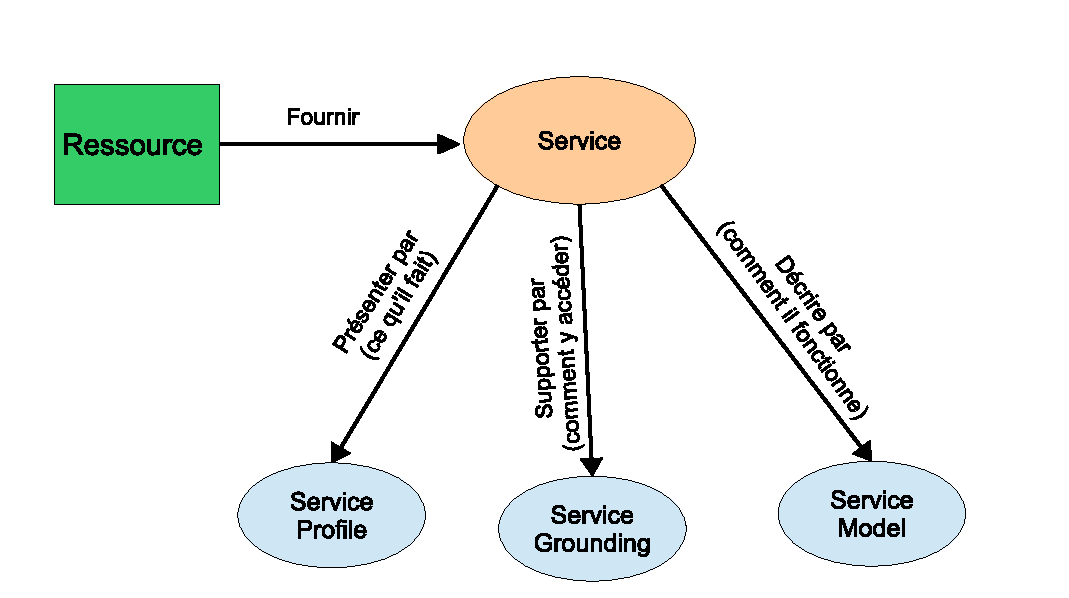
\includegraphics[width=0.8\textwidth]{figs/owls.eps}
    \caption{Les éléments d'une ontologie \textsc{OWL-S}}
    \label{fig:owl-s}
\end{figure}


    L'objectif principal de ces recherches est d'établir une
    plateforme dans laquelle les descriptions des services Web sont
    partagés en utilisant une ontologie standard, constituée d'un
    ensembles de classes de base et des propriétés pour résoudre les
    ambiguïtés et de rendre la description d'un service compréhensible
    par une machine.\newpage

    la figure \ref{fig:owl-s} décrit la structure tripartie d'une
    ontologie \textsc{OWL-S}. Elle est composé de trois
    sous-ontologie: un \emph{service profile}, d'un \emph{service
      model} et d'un \emph{service grounding}.

    \SpecialItem
    \begin{description}
    \item[ServiceProfile.] il offre une description informelle des
      fonctionnalités rendues par le service (\verb|serviceName|,
      \verb|textDescription|) et des informations concernant son
      fournisseur (\verb|contactInformation|). D'une aure côté, il
      spécifie des fonctionnalités offertes par le service (
      comportement fonctionnel) en terme de transformation
      d'information dénotée par les \textit{Entrés/Sorties}
      \textsc{(I/O)} (\verb|hasInput|, \verb|hasOutput|) et de
      changement d'état après l'exécution du service dénoté par les
      \textit{pré-conditions/effets} \textsc{(P/E)}
      (\verb|hasPrecondition|, \verb|hasResult|).

      Du point de vue de découverte et de la composition, Le
      \verb|ServiceProfile| est la partie la plus importante de la
      définition du service \textsc{OWL-S}.

    \item[ServiceModel.] il décrit le fonctionnement du service du en
      indiquant comment les résultats sont produits étape par étape
      précisant la façon un client peut interagir avec le service afin
      d'atteindre sa fonctionnalité. Ceci est fait en exprimant la
      transformation de données avec \textit{Entrés/Sorties}
      \textsc{(I/O)} etla transformation de l'Etat avec
      \textit{pré-conditions/effets} \textsc{(P/E)}.

      le \verb|ServiceProfile| est généralement considéré comme un
      sous-ensemble du \verb|ServiceModel|, contenant uniquement
      l'information nécessaire pour annoncer le service Web pour une
      découverte ultérieure.

    \item[ServiceGrounding.] Permet de spécifier les détails d'accès
      au service en précisant le protocole, le format des messages, la
      sérialisation et l'adressage. Il représente une correspondance
      \textit{(mapping)} entre la définition abstraite d'un processus
      \textsc{OWL-S} décrivant le service et la définition
      \textsc{WSDL} concrète des éléments nécessaires pour interagir
      avec le service.

      Le rôle de mise en correspondance est principalement à de
      combler l'écart entre la description sémantique des services Web
      (détallée dans le deux premières sous-ontologies) et les
      modèles de description de service existants qui sont
      principalement syntaxique (\textsc{WSDL}).
    \end{description}

    Le \verb|ServiceProfile| fournissent éventuellement d'autres
    informations supplémentaires sur le service comme la qualité
    qu'il assure en terme du temps de réponse et du coût, une
    classification possible d'un service \\(\verb|serviceCategory|),
    et un paramètre générique \verb|serviceParameter|.
    \\
    {\color{red}

      \begin{description}
      \item[Le processus atomique] directement invoqué par
        l’intermédiaire d’un Grounding
      \item[Le processus composé] décomposable en d’autres processus
        plus simples en utilisant les commandes de contrôle (par
        exemple : Si-Alors-Sinon, ...)

      \item[Le processus simple] non-invoquable, il fournit simplement
        une vue d’un processus atomique ou une représentation
        simplifié d’un processus composé.
      \end{description}

      Les composants principaux d’un modèle de processus sont
      l’ontologie de processus (Process Ontology) et l’ontologie de
      contrôle du processus (Process Control Ontology).  L’ontologie
      de processus, décrit un service en termes d’IOPE. Cette
      ontologie peut être utilisée afin de supporter l’invocation et
      la composition automatique de services web.  L’ontologie de
      contrôle de processus décrit chaque processus comme étant un
      état en prenant en compte son activation, son exécution et sa
      terminaison.

      Nous pouvons constater que le langage OWL-S s'adapte bien au
      besoin des méthodes de planification qui exigent une description
      de l’état du monde avant et après l’exécution d’un service donné.

      Any language is barely practical if its usage is not supported
      by tools. Several tools are proposed to create, or manipulate
      the OWL-S descriptions of services.  The most usable are OWL-S
      API, WSRF2OWLS, JAX-SA (Bab  et al., 2006, ık 2007; Habala et
      al., 2006). JAX-SA is an enhancement of WSRF2OWLS. The tool
      provides an interface on the top of the OWL-S API to create
      OWL-S service descriptions. The OWL-S generation process is
      semi-automatic. It requires a man- ually created configuration
      file depicting the mapping between the I/O parameters defined in
      WSDL and the ontological classes defined in OWL. Based on this,
      it automatically generates the semantic annotation. The
      disadvantage of all the tools is a lack of support to describe
      the pre-/post-conditions.\cite{bartalos2011effective}

      nous montrons dans la section suivante qu’elle présente des
      limitations pour en décrire les aspects non
      fonctionnels.\cite{jean2012prise}

      \begin{itemize}
        \item les limitaion de OWLS \cite{jean2012prise}
        \item d'augmentation de OWLS par QoS \cite{baryannis2010},
          \cite{kritikos2009requirements}
      \end{itemize}
    }
    \newpage
    \subsection{Comparaison}
    \label{sec:langs-comparaison}

    Une composition des services Web nécessite la satisfaction de
    plusieurs exigences techniques (\cite{sheng2014web}
    \cite{bucchiarone2006survey}) , le tableau
    \ref{comparaison-des-standards-et-langages-d-composition} montre
    une comparaison entre les langages et standards étudiées dans
    cette section selon les critères suivants:
    \begin{table}[htb!]
  \centering
  \begin{tabular}{|lcccc|}
    \hline
    \head{Langages}& \textsc{BPLE} & \textsc{WS-CDL} & \textsc{WSFM} & \textsc{OWL-S}\\
    \hline\hline
    \textbf{Composabilité} &\verb|+|& \verb|+|&\verb|-|&\verb|+|\\
    \textbf{Representation du rôle} &\verb|+|& \verb|+|&\verb|-|&\verb|-|\\
    \textbf{Support des structures complexes} &\verb|+|& \verb|+|&\verb|-|&\verb|+|\\
    \textbf{Compensabilité} &\verb|+|& \verb|+|&\verb|-|&\verb|-|\\
    \textbf{Support du sémantique} &\verb|-|& \verb|-|&\verb|+|&\verb|+|\\
    % TODO réviser critères
    \textbf{Support industriel} &\verb|+|& \verb|-|&\verb|-|&\verb|+|\\
    \hline
  \end{tabular}
  \newline

  \raggedright
  (\verb|+|) support, (\verb|-|) pas du support.
  \caption{Comparaison des standards et langages de composition}
  \label{comparaison-des-standards-et-langages-d-composition}
\end{table}
%%% Local Variables:
%%% mode: latex
%%% TeX-master: "../main"
%%% End:

    \SpecialItem
    \begin{itemize}
      \item [La composabilité] indique la capacité
        d'assembler des services participants dans un processus de
        composition et de modéliser les interactions entre eux.

      \item [La representation du rôle] indique La représentation de
        rôle indique la capacité de refléter la le comportement que le
        participant doit présenter afin d'interagir dans le processus
        de composition.

      \item [Le support des structures complexes] la capacité de
        modéliser les structures complexes qui reflètent les règles
        des actions réalisées dans le processus de composition logique
        d'exécution et de commande.

      \item [Compensabilité] est la capacité de gérer les
        exceptions de processus lors de l'exécution du processus de
        composition

      \item [le support du sémantique] est la capacité de représenter
        la sémantique de services participants pour faciliter la
        découverte des services et la composition dynamique.

      \item [le support industriel] indiqué par la qualité des outils
        et le support industriel de la technologie.
    \end{itemize}

    % TODO expand the table here for more details + conclude this
    % subsection

    % gives a detailed language capacity comparison of BPEL, WS-CDL,
    % BPML, ebXML, OWL-S, and WSMF. From Table 1, we can see that all
    % languages except WSMF support the modeling of message exchanging
    % and complex structure. Only BPEL and WS-CDL have the comprehensive
    % expressibility to define interacting roles, complex structures,
    % exception handling and compensation management. BPML does not
    % support role representation and ebXML does not provide a
    % compensation mech- anism. We also can observe that only OWL-S and
    % WSMF provide semantic support for services composition.

  \section{Les approches de composition dynamiques des services web}
  \label{sec:comp-dynam}

  La littérature quit traite la problématique de composition des
  services comporte une multitude d'approches visant à décrire
  l'interaction entre les services afin construire de nouveaux
  services composites répondant à un objectif donné. Selon l'approche
  proposée, les interprétations différent de ce que devraient être
  traitées dans une approche de composition, Ils diffèrent également
  sur le degré d'automatisation impliqué dans le processus allant des
  approches semi-automatisées à entièrement automatisés.

  Dans cette section, nous allons décrire et classifier les approches
  principales de composition proposées par différents auteurs issues
  de plusieurs communautés de recherches. La classification présentée
  par la suite est basée essentiellement sur l'état de l'art fait par
  Baryannis \emph{et al.}\cite{baryannis2010}.Nous distinguons quatres
  catégories de composition dynamique des services Web:
  \SpecialItem
  \begin{description}
  \item[La composition  basée sur les workflows]: Ces approches
    éxploitent les résultats des recherches dans le domaine des
    \textit{workflows}.

  \item[La composition dirigée par les modèles]: Ces approches
    utilisent les languages de modélisation (les réseux de Petri,
    \textsc{UML}) pour décrire la composition des services.

  \item[La composition algébrique et mathématique des services web]:
    Ces approches utilisent des méthodes mathématiques (logique
    mathématiques, algèbre).

  \item[La composition basée sur les techniques de planification]: Ces
    approches traitent le problème de composition comme un problème de
    planification.
  \end{description}

  \subsection{La composition  basée sur les workflows}
    \label{sec:les-approches-basees}
    Appuyant principalement du fait qu'un service composite est
    conceptuellement similaire à un \textit{workflow}, il est possible
    d'exploiter les connaissances accumulées dans la communauté de
    \textit{workflow} afin de faciliter la composition de services
    Web. Un \textit{workflow} est un flux d'informations au sein d'une
    organisation, tel que la transmission de documents entre les
    personnes. Il modélise une séquence d'opérations, réalisées par
    différentes entités au sein de l'organisation. Pratiquement, un
    \textit{workflow} est considéré comme la modélisation d'un
    ensemble de tâches, accomplies par différents acteurs impliqués
    dans la réalisation d'un processus métier. La modélisation de la
    composition de services sous forme d'un processus métier est de
    plus en plus populaire.

    Les approches de composition des services Web basées sur les
    techniques de \textit{workflow} étaient l'une des prmières
    solutions proposées pour la composition automatiques des services
    Web. Initialement, la plupart des travaux ont porté sur la
    composition statique et manuelle. Des travaux plus récents,
    cependant, a tenté de réaliser la composition dynamiques des
    services Web. En raison de la popularité de \textsc{BPEL} dans le
    milieu industriel, la plupart des approches dans cette catégorie
    emploient \textsc{BPEL} d'une manière ou d'une autre.

    %% TODO
    Majithia \textit{et al.} \cite{majithia2004framework} présentent
    une plateforme de construction automatique des schémas de
    composition.

    %% TODO
    \textit{Paws} \cite{ardagna2007paws} est une plateforme de
    composition des services Web qui se concentre sur l'adaptabilité et
    la flexibilité d'une composition modélisé sous forme un processus
    métier.

    %% TODO
    fujii et \textit{et al.} \cite{fujii2006semantics}
    \cite{fujii2009semantics} proposent une architecture.

    En générale, nous pouvsons conclure que même si les apprcohes de
    composition à base de \textit{workflow} ont évolué afin de
    supporter la composition automatique, les résultats sont limitées
    à des schémas de composition simples tels que l'éxécution
    séquentielle et parallèles. Cette lacune a été comblée en
    combinant méthodes à base de \textit{workflow} avec des techniques
    de planification issues du domaine d'intélégence artificielle. Ces
    approches serons éxaminer dans la quatrième catégorie
    \ref{sec:techn-de-plan}.

    \subsection{La composition dirigée par les modèles}
    \label{sec:model-based-composition}

    L'ingénierie dirigée par les modèles \acrshort{mdo} est une
    méthodologie de développement logiciel où l'accent est mis sur la
    création de modèles abstraits, indépendants de la plateforme et de
    la technologie. Un paradigme de modélisation doit fournir des
    modèles logiques du point de vue de l'utilisateur tout en restant
    suffisamment précis pour servir de base à l'implémentation
    \cite{dumez2010approche}. Les approches dans cette catégorie
    utilisent des méthodes déjà explorées et des modèles bien établis
    pour représenter un système de composition afin de pâlir la
    complexité croissante de cette dernière utilisant une description
    plus abstraite au dessus de la description traditionnelle de
    services dans \textsc{WSDL}, \textsc{OWL-S} ou similaire.

    \textsc{UML}\footnote{\url{http://www.omg.org/spec/UML/}}
    \cite{rumbaugh2004unified} est un langage de modélisation maintenu
    par l'\textsc{OMG}\footnote{\url{http://www.omg.org}} qui s'est
    standardisé de par sa position dominante dans l'industrie du
    logiciel. \textsc{UML} est un langage polyvalent permettant de
    modéliser un système selon différents points de vue, Le point de
    vue statique ou structurel du système et le point de vue dynamique
    représente le comportement dynamique d'un système en montrant les
    interactions entre les objets ou les changements d'états au sein
    d'un objet.

    Skogan \textit{et al.}  \cite{skogan2004web} proposent une méthode
    qui utilise les diagrammes d'activités \textsc{UML} pour modéliser
    la composition des services. Ces diagrammes là sont utilisés pour
    générer un processus exécutable d'orchestration \textsc{BPEL}
    utilisant des transformations \textsc{XSLT}, ce tarvail se limite
    à la description syntaxique de service Web utilisant les documents
    \textsc{WSDL} comme des entrées de la transformation
    \textsc{UML}. Dans \cite{gronmo2005model} les auteurs essayent de
    soulèver cette limitation en considérant également
    l'enrichissement sémantique des services avec des ontologies
    \textsc{OWLS} et des annotations \textsc{WSMO}.

    Les réseaux de Petri \cite{petri1962kommunikation} constituent une
    approche bien établie pour la modélisation de processus. Un réseau
    de Petri est un graphe dirigé, connecté et biparti qui représente
    les transitions entre plusieurs états du système, ainsi que les
    ressources disponibles \cite{dumez2010approche}.

    Hamadi et Benatallah dans \cite{hamadi2003petri} proposent une
    méthode de modélisation basée sur les réseaux de Petri pour
    modéliser le flux de contrôle et la sémantique des compositions de
    services en assignant une transition à chaque appel de service et
    une place à chaque état entre les appels, chaque service composite
    est modélisé par un réseau de Petri contenant un état d'entrée et
    de sortir permettant de modéliser respectivement la réception et
    l'émission d'informations par le service composite. Dans
    \cite{ouyang2007formal} les auteurs présentent une traduction
    complète de \textsc{BPEL} en réseaux de Petri permettant la
    vérification automatique des processus \textsc{BPEL}.

    \subsection{La composition algébrique et mathématique}
    \label{sec:les-apprc-math}
    Cette catégorie d'approches inclues toutes les approches ont la
    caractéristique commune à être fondée sur des bases mathématiques
    tels que le logique temporelle et linéaire, calcule formel,
    calcule algébrique des processus et autres méthodes
    mathématiques. De nombreux langages, présentés comme des algèbres
    de processus, ont été développés pour une compréhension formelle
    et la spécification d'applications à services \textsc{SOA}. les
    langages d'orchestration tels que \acrshort{xlang} et
    \acrshort{bpel} ont fortement inspirés de la métaphore de
    communication inspirée du $\pi$-calcule basé sur l'échange de
    messages dans un contexte distribué.

    Les algèbres de processus sont des formalismes de description
    formelle pour la spécification de systèmes logiciels, en
    particulier pour les systèmes concurrentiels
    \cite{dumez2010approche}. Elles fournissent des outils pour la
    description de haut niveau des interactions et des
    synchronisations entre les processus. Plusieurs algèbres de
    processus ont été décrites. Parmi les plus anciennes on peut citer
    \acrshort{csp} qui a été présenté par Hoare
    \cite{hoare1978communicating}, \acrshort{ccs} qui a été proposé
    par Milner \cite{milner1982finite}, \cite{milner1989communication}
    et le $\pi$-calcule \cite{milner1992calculus}.

    Milanovic \textit{et al.} \cite{milanovic2004current} montre que
    L'utilisation des langages algébriques de processus et langages
    formels, comme le \textsc{CCS} et le $\pi$-calculusa été
    préconisée pour la composition de services Web, car les
    spécifications de processus comprises dans les standards des
    services Web comme \acrshort{wsmo} ou \acrshort{wsmf} sont
    formellement fondées sur le algèbre des processus.

    La composition algébrique permet modéliser les services comme des
    processus mobiles pour assurer une vérification de certaines
    propriétés tel que l'éxactitude, la sécurité, la vivacité
    \textit{(liveness)}, et la gestion des ressources. La théorie des
    processus mobiles est basée sur le $\pi$-calcule, dans laquelle
    l'entité de base est un processus qui peut être un processus vide,
    un choix (branchement) entre plusieurs opérations
    d'\textit{Entrés/Sorties} et leurs continuations, une composition
    parallèle, une définition récursive, ou une invocation récursive
    \cite{zahirathesis2008}.

    Dans \cite{koshkina2004modelling}, la sémantique du langage de
    chorégraphie \textsc{WS-CDL} est décrite à l'aide de \textsc{CSP}
    pour permettre la vérification automatiques de propriétés. Un
    travail similaire est réalisé dans \cite{li2007modeling} où des
    règles sont présentées pour traduire chaque construction
    syntaxique de \textsc{WS-CDL} en \textsc{CSP}.

    Rao \textit{et al.} \cite{rao2004logic} proposent l'utilisation de
    la logique linéaire pour la composition automatique des services
    Web. La logique linéaire est une extension de la logique classique
    de premier ordre pour modéliser la notion d'évolution d'états. les
    auteurs proposent une méthode de traduction automatique de
    descriptions \textsc{OWL-S} à des axiomes de la logique
    linéaire. Ensuite, ils utilisent la démonstration automatique des
    théorèmes pour produire des schémas abstraits de composition, qui
    sont ensuite transformés à des modèles de \textit{workflows}
    \textsc{BPEL} en utilisant un langage d'algèbre des processus
    inspiré par le $\pi$-calcule.

    \subsection{La composition basée sur les techniques de planification}
    \label{sec:techn-de-plan}
    Selon \cite{baryannis2010}, \cite{bartalos2011effective},
    \cite{chan2007survey}, \cite{peer2005web}, \cite{rodriguez2011automatic}
    % \newpage

  \section{Conclusion}
  \label{sec:conclusion}
  Introduire la composition dynamique basé sur le modèle graphe qui se
  sera détaillé dans le prochain chapitre.
  % TODO rapeller du problème initiale en contexte de ce chapitre

%%% Local Variables: 
%%% mode: latex
%%% TeX-master: "../main"
%%% End:
